\documentclass[tikz, border=12pt]{standalone}
\usepackage{amsmath}
\usetikzlibrary{positioning, arrows.meta, calc}
\begin{document}
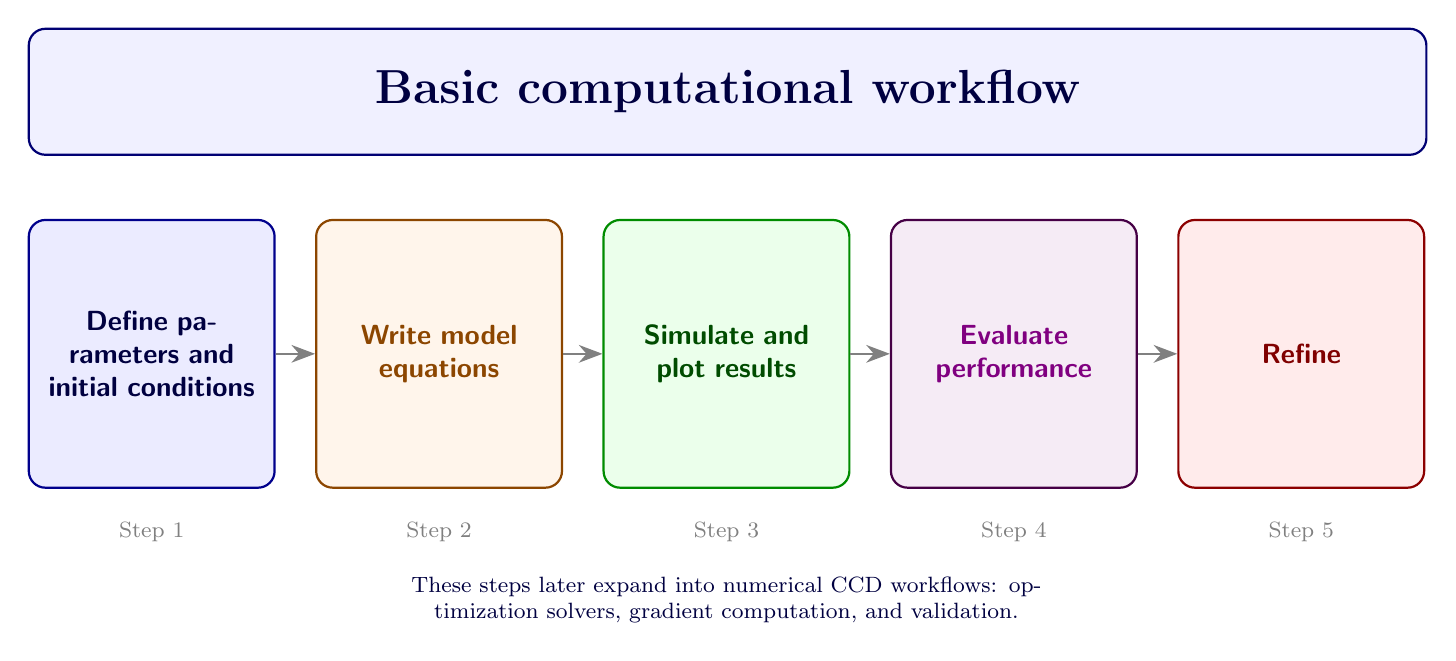
\begin{tikzpicture}[
    font=\sffamily,
    node distance=8mm and 5mm,
    card/.style={rectangle, rounded corners=6pt, draw=#1!55!black, thick,
        fill=#1!8, minimum width=3.0cm, minimum height=3.4cm,
        text width=2.7cm, align=center, inner sep=6pt},
]

% ---- Cards placed first ----
\node[card=blue, anchor=north west] (s1) at (0,0)
    {\textcolor{blue!25!black}{\bfseries Define parameters and initial conditions}};
\node[card=orange, right=of s1] (s2)
    {\textcolor{orange!55!black}{\bfseries Write model equations}};
\node[card=green,  right=of s2] (s3)
    {\textcolor{green!30!black}{\bfseries Simulate and plot results}};
\node[card=violet, right=of s3] (s4)
    {\textcolor{violet}{\bfseries Evaluate performance}};
\node[card=red,    right=of s4] (s5)
    {\textcolor{red!50!black}{\bfseries Refine}};

% ---- Title box: width computed exactly to span s1.west -> s5.east ----
\path let \p1 = (s1.west), \p2 = (s5.east), \p3 = (s1.north) in
    node[draw=blue!45!black, thick, rounded corners=6pt, fill=blue!6,
         minimum width={\x2-\x1}, minimum height=1.6cm, align=center,
         font=\bfseries\LARGE, text=blue!25!black, anchor=south west]
        (title) at (\x1,{\y3+8mm}) {Basic computational workflow};

% ---- Arrows between cards ----
\draw[-{Stealth[length=3mm]}, thick, gray] (s1.east) -- (s2.west);
\draw[-{Stealth[length=3mm]}, thick, gray] (s2.east) -- (s3.west);
\draw[-{Stealth[length=3mm]}, thick, gray] (s3.east) -- (s4.west);
\draw[-{Stealth[length=3mm]}, thick, gray] (s4.east) -- (s5.west);

% ---- Step labels ----
\node[below=3mm of s1.south, font=\footnotesize, text=gray] {Step 1};
\node[below=3mm of s2.south, font=\footnotesize, text=gray] {Step 2};
\node[below=3mm of s3.south, font=\footnotesize, text=gray] {Step 3};
\node[below=3mm of s4.south, font=\footnotesize, text=gray] {Step 4};
\node[below=3mm of s5.south, font=\footnotesize, text=gray] {Step 5};

% ---- Caption ----
\node[below=10mm of s3.south, text width=13.5cm, align=center, font=\footnotesize]
    {\textcolor{blue!25!black}{These steps later expand into numerical CCD workflows: optimization solvers, gradient computation, and validation.}};

\end{tikzpicture}
\end{document}
